\documentclass{article}

% includes for math symbols
\usepackage{amsmath}
\usepackage{amssymb}
% required packages for the figure and table macros of texenv.
% the docstring for each macro should list the required packages. 
\usepackage[table]{xcolor}
\usepackage{graphicx}

\usepackage[margin=1.5in]{geometry}

\setlength{\parindent}{0pt}

\begin{document}

\section{PEC Edge Singularity Treatment}

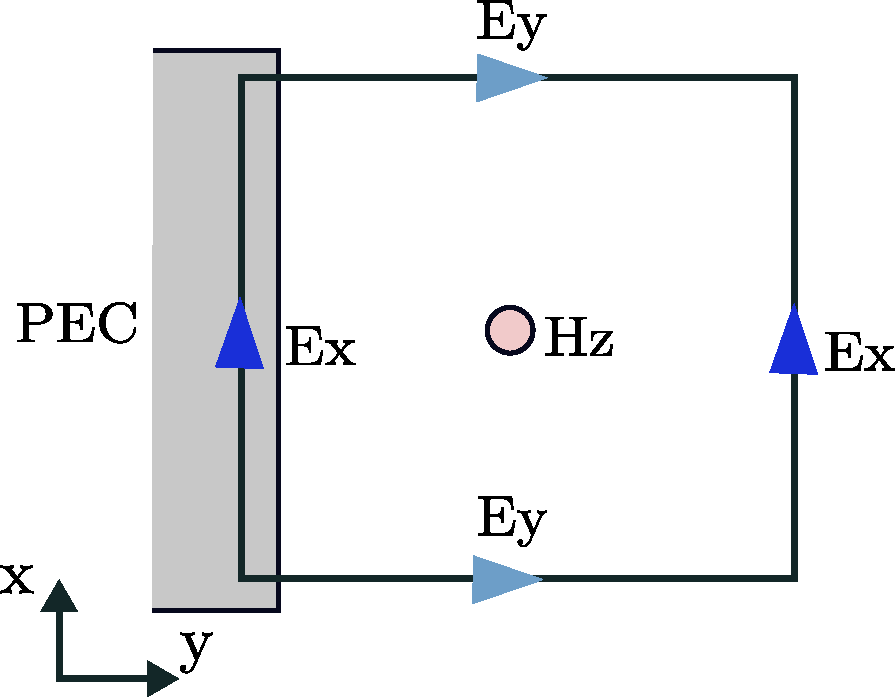
\includegraphics[width=3in]{ms_edge.pdf}

\vspace{0.2in}

\(H_z\) and \(E_y\) vary as \(1 / r\).

For the Hz, update, instead of linearly interpolating the \(E_x\) fields on either side, use the \(1 / r\) model.


The \(H_z\) field at a distance \(r\) from the PEC edge is,
\[H_z(r) = {H_{z0} \over r}\]

The constant \(H_{z0}\) can be found since the field at \(\Delta y \over 2\) is the \(H_z(i,j,k)\) component in the Yee grid,
\[H_z\Big(r={\Delta y \over 2}\Big) = {2 H_{z0} \over {\Delta y}} = H_z(i,j,k) \]

\[H_{z0} = { H_z(i,j,k) \Delta y \over 2 } \]

So the \(H_z\) at any point \(r\) is,
\[H_z(r) = { H_z(i,j,k) \Delta y \over 2 r}\]

By similar logic, since \(E_y\) is at the same point along r as \(H_z\),
\[E_y(r) = { E_y(i,j,k) \Delta y \over 2 r}\]

Plugging this in to the update equation for \(H_z\),
\[\mu_0 \int_S {\partial H_z \over \partial t} dS = \Big[E_x(i, j+1, k) - E_x(i, j, k)\Big] \Delta x - \int_{r=a}^{r=\Delta y}\Big[E_y(i+1, k) - E_y(i, k)\Big] dr \] 

\[\mu_0 \int_{x=0}^{x=\Delta x} \int_{r=a}^{r=\Delta y}{\partial \over \partial t}  { H_z(i,j,k) \Delta y \over 2 r} dxdr =\]
\[+ \Big[E_x(i, j+1, k) - E_x(i, j, k)\Big] \Delta x\]
\[- \int_{r=a}^{r=\Delta y}\Big[{ E_y(i+1,j,k) \Delta y \over 2 r} - { E_y(i,j,k) \Delta y \over 2 r}\Big] dr \] 


Evaluating the first term,
\[\mu_0 \int_{x=0}^{x=\Delta x} \int_{r=a}^{r=\Delta y}{\partial \over \partial t}  { H_z(i,j,k) \Delta y \over 2 r} dxdr =\]
\[ \Delta x \mu_0 { \partial H_z(i,j,k)  \over \partial t} { \Delta y \over 2 } \log(r)\Big|_{r=a}^{r=\Delta y}\]
\[= \Delta x \mu_0  { \Delta y \over 2 } \log\Big({\Delta y \over a}\Big) { \partial H_z(i,j,k)  \over \partial t}\]

The \(E_y\) terms are similar,
\[- \int_{r=a}^{r=\Delta y}\Big[{ E_y(i+1,j,k) \Delta y \over 2 r} - { E_y(i,j,k) \Delta y \over 2 r}\Big] dr \] 
\[= - \Big[{ E_y(i+1,j,k) } - { E_y(i,j,k) }\Big] {\Delta y \over 2} \log\Big({\Delta y \over a}\Big)  \] 

The full update equation is then,
\[ \Delta x \mu_0  { \Delta y \over 2 } \log\Big({\Delta y \over a}\Big) { \partial H_z(i,j,k)  \over \partial t}=\]
\[+ \Big[E_x(i, j+1, k) - E_x(i, j, k)\Big] \Delta x\]
\[ - \Big[{ E_y(i+1,j,k) } - { E_y(i,j,k) }\Big] {\Delta y \over 2} \log\Big({\Delta y \over a}\Big)  \] 

Applying central differencing to the \(H_z\) term,
\[ \Delta x \mu_0  { \Delta y \over 2 } \log\Big({\Delta y \over a}\Big) { H_z^{n+1}(i,j,k) -H_z^{n}(i,j,k)  \over  \Delta t}=\]
\[+ \Big[E_x(i, j+1, k) - E_x(i, j, k)\Big] \Delta x\]
\[ - \Big[{ E_y(i+1,j,k) } - { E_y(i,j,k) }\Big] {\Delta y \over 2} \log\Big({\Delta y \over a}\Big)  \] 

Solving for \(H_z^{n+1}\),
\[ H_z^{n+1}(i,j,k) =  H_z^{n}(i,j,k) + \]
\[ \Big[E_x(i, j+1, k) - E_x(i, j, k)\Big] {2 \Delta t\over \mu_0 \Delta y \log\Big({\Delta y \over a}\Big) }\]
\[ - \Big[{ E_y(i+1,j,k) } - { E_y(i,j,k) }\Big] {\Delta t\over \mu_0 \Delta x }  \] 

% For the \(E_y\) components,

% \[{\partial E_y \over \partial t} = { 1 \over \epsilon} \Big[ {\partial H_x \over \partial z} - {\partial H_z \over \partial x} \Big]\]


% \[{\partial H_z \over \partial t} = { 1 \over \mu} \Big[ {\partial E_x \over \partial y} - {\partial E_y \over \partial x} \Big]\]

\end{document}